\documentclass{article}
\usepackage{amsfonts, amsmath, amssymb, amsthm} % Math notations imported
\usepackage{enumitem}
\usepackage{graphicx}
\usepackage{setspace}
\usepackage{indentfirst}
\usepackage[margin=1in]{geometry}
\graphicspath{{./images/}} % Path to images

% \begin{figure}[htb!]
%      \centering
%      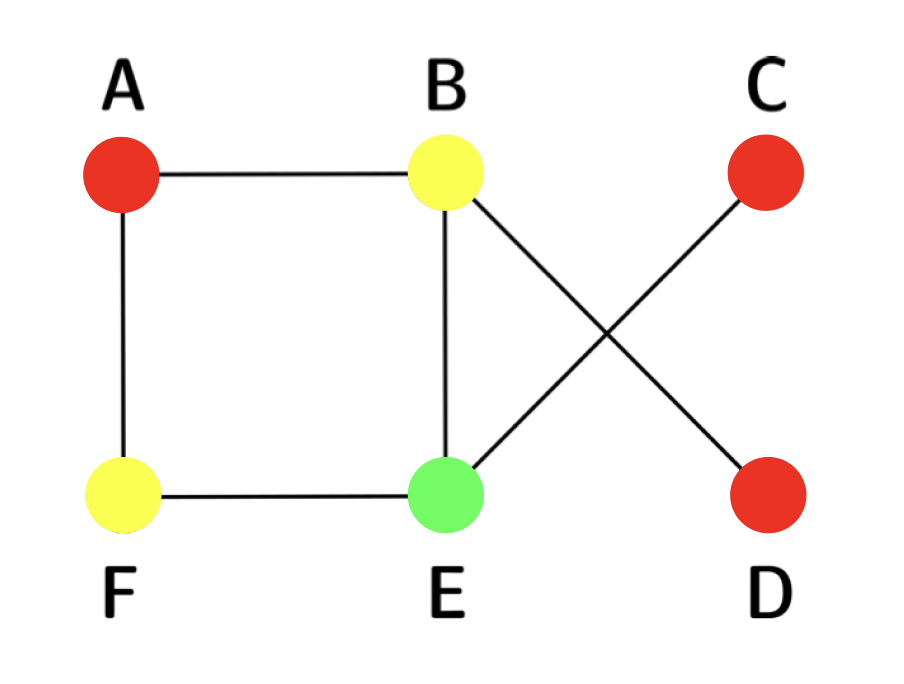
\includegraphics[scale=0.5]{coloring.png}
%      \caption{Coloring of the graph.}
% \end{figure}

% \begin{figure}[htb]
%     \qquad
%     \begin{minipage}{.4\textwidth}
%         \centering
%         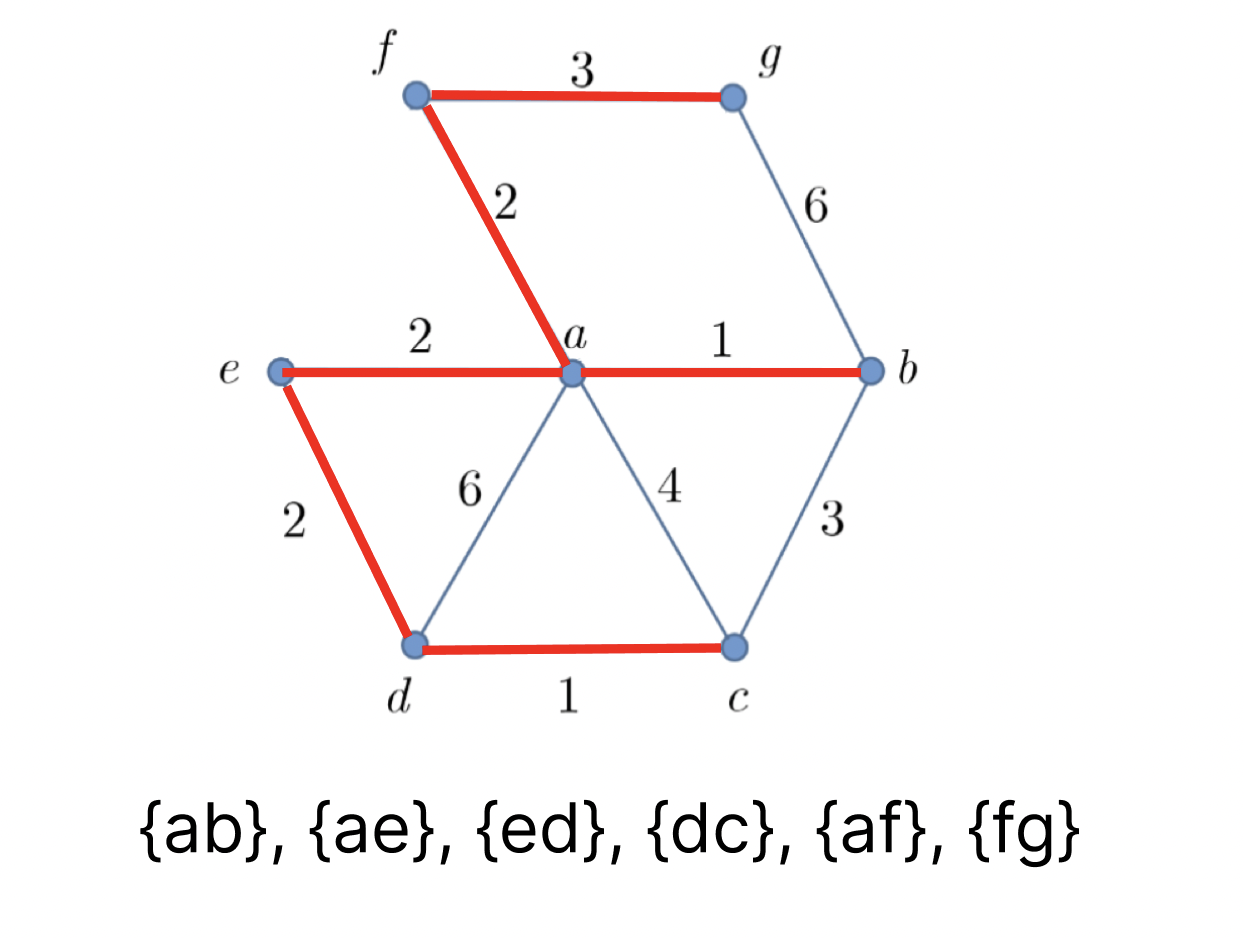
\includegraphics[scale=0.35]{prims.png}
%         \caption{}
%     \end{minipage}    
%     \qquad
%     \begin{minipage}{.4\textwidth}
%         \centering
%         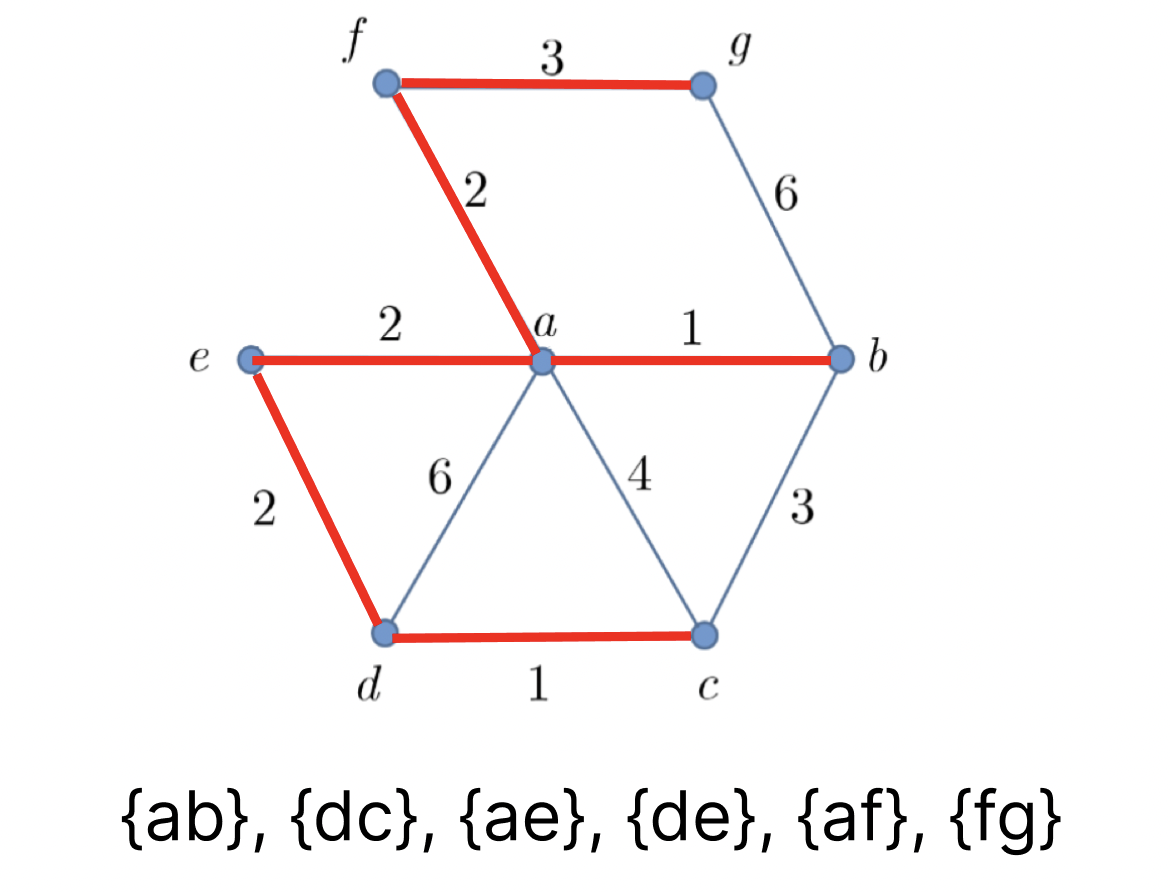
\includegraphics[scale=0.35]{kruskal.png}
%         \caption{}
%     \end{minipage}        
% \end{figure} 

\newtheorem{thm}{Theorem}
\newtheorem{proposition}[thm]{Proposition}
\newtheorem{cor}[thm]{Corollary}

% title information
\title{Math 109 HW}
\author{Neo Lee}
\date{MM/DD/YYYY}

\setstretch{1.15}
% main content
\begin{document} 

% placing title information; comment out if using fancyhdr
\maketitle 

\textbf{With intercept:}
Define $$Q := \mathbb{E} \big[ (y - \beta_0 - \beta_1 x)^2 \big].$$ Then we have
\begin{align*}
    \frac{\partial Q}{\partial \beta_0} = \mathbb{E} \big[2 (\beta_0 + \beta_1 x - y) \big] & = 0 \\
    2 \mathbb{E}\big[\beta_0 \big] + 2 \mathbb{E}\big[\beta_1 x \big] - 
    2 \mathbb{E}\big[y \big] & = 0 \\
    \beta_0 + \beta_1 \mu_x - \mu_y & = 0 \\
    \underline{\beta_0} & = \mu_y - \beta_1 \mu_x.
\end{align*}
Then, we can find $\beta_1$ by setting
\begin{align*}
    \frac{\partial Q}{\partial \beta_1} = \mathbb{E} \big[2 x (\beta_0 + \beta_1 x - y) \big] & = 0 \\
    \beta_0\mathbb{E}\big[y \big] + \beta_1\mathbb{E}\big[x^2 \big] - \mathbb{E}\big[xy \big] & = 0 \\
    \beta_0\mu_x + \beta_1\left(Var(x)+\mu_x^2\right) - \left(Cov(x,y) + \mu_x\mu_y\right) & = 0 \\
    (\mu_y - \mu_x\beta_1)\mu_x + \beta_1Var(x) + \beta_1\mu_x^2 - Cov(x,y) - \mu_x\mu_y & = 0 \\
    \beta_1Var(x) - Cov(x,y) & = 0 \\
    \underline{\beta_1} & = \frac{Cov(x,y)}{Var(x)}.
\end{align*}

Define $$Q:=\mathbb{E}\left[(y-\beta_1x)^2\right].$$
Then we have
\begin{align*}
    \frac{\partial Q}{\partial \beta_1} = \mathbb{E} \big[2 x (\beta_1 x - y) \big] & = 0 \\
    \beta_1\mathbb{E}\big[x^2 \big] - \mathbb{E}\big[xy \big] & = 0 \\
    \beta_1\left(Var(x)+\mu_x^2\right) - \left(Cov(x,y) + \mu_x\mu_y\right) & = 0 \\
    \underline{\beta_1} & = \frac{Cov(x,y)+\mu_x\mu_y}{Var(x)+\mu_x^2}.
\end{align*}

With intercept:

Define $$Q := \sum_{i=1}^n (y_i - \beta_0 - \beta_1 x_i)^2.$$

To find $\beta_0$, we set
\begin{align*}
    \frac{\partial Q}{\partial \beta_0} = \sum 2(\beta_1x_i+\beta_0-y_i) & = 0 \\
    \sum\beta_1x_i + n\beta_0-\sum y_i & = 0 \\
    \beta_1\frac{1}{n}\sum x_i + \beta_0 - \frac{1}{n}\sum y_i & = 0 \\
    \beta_0 & = \frac{1}{n}\sum y_i - \beta_1\frac{1}{n}\sum x_i \\
    \beta_0 & = \bar{y} - \beta_1\bar{x}.
\end{align*}

To find $\beta_1$, we set
\begin{align*}
    \frac{\partial Q}{\partial \beta_0} = \sum 2x(\beta_1x_i+\beta_0-y_i) & = 0 \\
    \beta_1\sum x_i^2+\beta_0\sum x_i - \sum x_iy_i & = 0 \\
    \beta_1\sum x_i^2 + \left(\bar{y} - \beta_1\bar{x}\right)\sum x_i - \sum x_iy_i & = 0 \\
    \beta_1\sum x_i^2 + \bar{y}\sum x_i - \beta_1\bar{x}\sum x_i - \sum x_iy_i & = 0 \\
    \beta_1\left(\sum x_i^2 - \bar{x}\sum x_i\right) & = \sum x_iy_i - \bar{y}\sum x_i \\
    \beta_1 & = \frac{\sum x_iy_i - \bar{y}\sum x_i}{\sum x_i^2 - \bar{x}\sum x_i}.
\end{align*}

Now, we take apart the numerator and denominator of $\beta_1$:
\begin{align*}
    \sum x_iy_i - \bar{y}\sum x_i & = \sum (x_iy_i) - \bar{y}\cdot n\bar{x} \\
    & = \sum (x_iy_i) - \bar{y}\cdot n\bar{x}  - \bar{x}\cdot n\bar{y} + n\bar{x}\bar{y} \\
    & = \sum (x_iy_i) - \bar{y}\sum x_i - \bar{x}\sum y_i + n\bar{x}\bar{y} \\
    & = \sum\left(x_iy_i - x_i\bar{y} - \bar{x}y_i + \bar{x}\bar{y}\right) \\
    & = \sum(x_i-\bar{x})(y_i-\bar{y}); \\
    \sum x_i^2 - \bar{x}\sum x_i & = \sum x_i^2 - \bar{x}\cdot n\bar{x} \\
    & = \sum x_i^2 - \bar{x}\cdot n\bar{x} - \bar{x}\cdot n\bar{x} + \bar{x}\cdot n\bar{x} \\
    & = \sum x_i^2 - \bar{x}\sum x_i - \bar{x}\sum x_i + n\bar{x}^2 \\
    & = \sum\left(x_i^2 - 2x_i\bar{x} + \bar{x}^2\right) \\
    & = \sum(x_i-\bar{x})^2.
\end{align*}

Hence, 
\begin{align*}
    \beta_1 & = \frac{\sum_{i=1}^n(x_i-\bar{x})(y_i-\bar{y})}{\sum_{i=1}^n(x_i-\bar{x})^2}.
\end{align*}

Without intercept:

Define $$Q:=\sum_{i=1}^n(y_i-\beta_1x_i)^2.$$

To find $\beta_1$, we set
\begin{align*}
    \frac{\partial Q}{\partial \beta_1} = \sum 2x(\beta_1x_i-y_i) & = 0 \\
    \beta_1\sum x_i^2 - \sum x_iy_i & = 0 \\
    \beta_1 & = \frac{\sum x_iy_i}{\sum x_i^2}.
\end{align*}

Population version:

We are interested in knowing whether $\beta_{y|x} = \beta_{x|y}^{-1}$ in a model withou intercept.
We can check this by multiplying $\beta_{y|x}$ and $\beta_{x|y}$ and check if the result is 1.
\begin{align*}
    \beta_{y|x} \times \beta_{x|y} & = \frac{Cov(x,y)+\mu_x\mu_y}{Var(x)+\mu_x^2} 
    \times \frac{Cov(x,y)+\mu_x\mu_y}{Var(y)+\mu_y^2} \\
    & = \frac{\mathbb{E}\left[xy\right]^2}{\mathbb{E}\left[x^2\right]\mathbb{E}\left[y^2\right]} \\
    & = \frac{\mathbb{E}\left[(xy)^2\right]-Var(xy)}{\mathbb{E}\left[x^2\right]\mathbb{E}\left[y^2\right]} \\
    & = \frac{Cov(x,y)+\mathbb{E}\left[x^2\right]\mathbb{E}\left[y^2\right]-Var(xy)}{\mathbb{E}\left[x^2\right]\mathbb{E}\left[y^2\right]}.
\end{align*}

Hence, it is only true when $Cov(x,y)=Var(xy)=0$, and is not true in general.

Sample version:

Similarly, we proceed by multiplying $\beta_{y|x}$ and $\beta_{x|y}$ and check if the result is 1.
\begin{align*}
    \beta_{y|x} \times \beta_{x|y} & = \frac{\sum x_iy_i}{\sum x_i^2} \times \frac{\sum x_iy_i}{\sum y_i^2}.
\end{align*}
We can see easily that the product is not 1 in general. Arbitrarily, take $(1,2)$ for $i=1$ and 
$(3,4)$ for $i=2$, the product is 0.98.


Consider a model with intercept, 
\begin{align*}
    \hat{\beta}_1 & = \frac{\sum_{i=1}^n(x_i-\bar{x})(y_i-\bar{y})}{\sum_{i=1}^n(x_i-\bar{x})^2} \\
    & = \frac{\sum_{i=1}^n(x_i-\bar{x})(y_i-\bar{y})}{\sqrt{\sum_{i=1}^n(x_i-\bar{x})^2}\sqrt{\sum_{i=1}^{n}(y_i-\bar{y})^2}}\times 
    \frac{\sqrt{\sum_{i=1}^{n}(y_i-\bar{y})^2}}{\sqrt{\sum_{i=1}^{n}(x_i-\bar{x})^2}},
\end{align*}
which is represented by the sample correlation times the ratio of response sample standard 
deviations over predictor sample standard deviations.

Therefore, one plausible explanation is that the sample standard deviation of father's height is 
significantly larger than that of mother's height. Hence, even the correlation between 
a father's height and their child's height is larger, the standard deviation of father's height 
may rescale $\hat{\beta}_1^{\emph{dad}}$ to a smaller value than $\hat{\beta}_1^{\emph{mom}}$.


We first show that $$\left(\sum_{i=1}^{n}x_ix_i^T\right)^{-1} = \left(X^TX\right)^{-1},$$
then we show that $$\sum_{i=1}^{n}x_iy_i = X^Ty.$$

Notation: Denote $x_j^{(i)}$ as the $j$-th feature of the feature vector $\vec{x}$ at time step $i$. The 
subscript is the feature index, and the superscript is the time step index.
We rewrite the equation as $$\left(\sum_{i=1}^{n}x^{(i)}x^{(i)^T}\right)^{-1} = \left(X^TX\right)^{-1}$$ to align with our notation.

We first check $\sum_{i=1}^{n}x^{(i)}x^{(i)^T}$. For each time step $i$, $x^{(i)}x^{(i)^T}$ will produce a $p\times p$ matrix, denote $\mathcal{P}^{(i)}$, 
where $$\mathcal{P}_{k,l}^{(i)} = x_k^{(i)}\cdot x_l^{(i)}.$$ Hence, the summation 
$\sum_{i=1}^{n}x^{(i)}x^{(i)^T} = \mathcal{P}$ is a $p\times p$ matrix of sum of all $\mathcal{P}^{(i)}$, for which 
$$\mathcal{P}_{k,l} = \sum_{i=1}^{n}x_k^{(i)}\cdot x_l^{(i)}.$$

Now, we check $X^TX$, denote $\mathcal{P}^*$. $X^T$ is a $p\times n$ matrix, and $X$ is a $n\times p$ matrix, so indeed their 
product will produce a $p\times p$ matrix. Notice the $k$-th row of $X^T$ represents the $k$-th feature vector of all $n$ time steps, which means 
$$X^T_{k,\cdot} = \left[x_k^{(1)}, x_k^{(2)}, \cdots, x_k^{(n)}\right].$$
The $l$-th column of $X$ represents the $l$-th feature of all $n$ time steps, which means
$$X_{\cdot,l} = \begin{bmatrix}
    x_{l}^{(1)} \\
    x_{l}^{(2)} \\
    \vdots \\
    x_{l}^{(n)}
  \end{bmatrix}.$$
Hence, the $k,l$-th entry of $X^TX$ is
\begin{align*}
    \mathcal{P}^*_{k,l} & = X^T_{k,\cdot}X_{\cdot,l} \\
    & = x_k^{(1)}x_l^{(1)} + x_k^{(2)}x_l^{(2)} + \cdots + x_k^{(n)}x_l^{(n)} \\
    & = \sum_{i=1}^{n}x_k^{(i)}\cdot x_l^{(i)},
\end{align*}
and we can see that $\mathcal{P}^* = \mathcal{P}\Rightarrow\mathcal{P}^{*^{-1}} = \mathcal{P}^{-1}$, 
which means $\left(\sum_{i=1}^{n}x^{(i)}x^{(i)^T}\right)^{-1} = \left(X^TX\right)^{-1}$.

Next, we show $$\sum_{i=1}^{n}x_iy_i = X^Ty.$$ Again, we rewrite the equation to match our notation:
$$\sum_{i=1}^{n}x^{(i)}y^{(i)} = X^Ty.$$
For each $i$,
\begin{align*}
    x^{(i)}y^{(i)} & = 
    \begin{bmatrix}
        x_1^{(i)} \\
        x_2^{(i)} \\
        \vdots \\
        x_p^{(i)}
      \end{bmatrix}y^{(i)} = 
    \begin{bmatrix}
        x_1^{(i)}y^{(i)} \\
        x_2^{(i)}y^{(i)} \\
        \vdots \\
        x_p^{(i)}y^{(i)}
      \end{bmatrix}
\end{align*}
Hence, $\sum_{i=1}^{n}x^{(i)}y^{(i)}$ is a $p\times 1$ vector, denote $\vec{v}$, and the $k$-th entry 
$$\vec{v}_k = \sum_{i=1}^{n}x_k^{(i)}y^{(i)}.$$

Now we check $X^Ty$. $X^T$ is a $p\times n$ matrix, and $y$ is a $n\times 1$ vector, so indeed their
product will produce a $p\times 1$ vector, denote $\vec{v}^*$. Notice the $k$-th row of $X^T$ represents the $k$-th 
feature vector of all $n$ time steps, which means 
$$X^T_{k,\cdot} = \left[x_k^{(1)}, x_k^{(2)}, \cdots, x_k^{(n)}\right].$$
$y$ is a vector of all $n$ time steps, which means
$$y = \begin{bmatrix}
    y^{(1)} \\
    y^{(2)} \\
    \vdots \\
    y^{(n)}
  \end{bmatrix}.$$
Indeed, the $k$-th entry of $\vec{v}^*$ is
\begin{align*}
    \vec{v}^*_k & = X^T_{k,\cdot}y \\
    & = x_k^{(1)}y^{(1)} + x_k^{(2)}y^{(2)} + \cdots + x_k^{(n)}y^{(n)} \\
    & = \sum_{i=1}^{n}x_k^{(i)}y^{(i)}.
\end{align*}
Therefore, $\vec{v}^* = \vec{v}$, which means $\sum_{i=1}^{n}x^{(i)}y^{(i)} = X^Ty$.

Reuse the formula we derived from question 2, we have 
$$\hat{\beta}_1 = \frac{\sum_{i=1}^{n}x_iy_i}{\sum_{i=1}^{n}x_i^2}.$$
Taking $x_i = 1$ for all $i$,
$$\hat{\beta}_1 = \frac{\sum_{i=1}^{n}y_i}{\sum_{i=1}^{n}1} = \frac{\sum_{i=1}^{n}y_i}{n} = \bar{y}.$$








Let's first find $\hat{x}_j^{-j}$ and $\hat{y}^{-j}$.

Notation: Denote $x_0$ as the constant feature vector, and $x_1$ as the actual meaningful feature 
vector. We will take $j = 1$ for the rest of this problem. Any superscript $^{-j}$ will mean 
dropping $x_1$, and this is not to be confused with $^{-1}$, the inverse.

$\hat{x}_1^{-j}$ is the residual of regressing $x_1$ on $X^{-j}$. Note: $X^{-j}$ is essentially $x_0$.
From question 7, we know that
$$\hat{\beta}_{x_1|x_0} = \bar{x}_1.$$
Hence, the residual of regressing $x_1$ on $X^{-j}$ is
\begin{align*}
    \hat{x}_1^{-j} & = x_1 - x_0\hat{\beta}_{x_1|x_0} \\
    & = x_1 - x_0\bar{x}_1 \\
    & = \begin{bmatrix}
        x_1^{(1)} - \bar{x}_1 \\
        x_1^{(2)} - \bar{x}_1 \\
        \vdots \\
        x_1^{(n)} - \bar{x}_1 
    \end{bmatrix}
\end{align*}

$\hat{y}^{-j}$ is the residual of regressing $y$ on $X^{-j}$. Note: $X^{-j}$ is essentially $x_0$.
From question 7, we know that
$$\hat{\beta}_{y|x_0} = \bar{y}.$$
Hence, the residual of regressing $y$ on $X^{-j}$ is
\begin{align*}
    \hat{y}^{-j} & = y - x_0\hat{\beta}_{y|x_0} \\
    & = y - x_0\bar{y} \\
    & = \begin{bmatrix}
        y^{(1)} - \bar{y} \\
        y^{(2)} - \bar{y} \\
        \vdots \\
        y^{(n)} - \bar{y} 
    \end{bmatrix}
\end{align*}

Now, we put everything together.
\begin{align*}
    \hat{\beta}_{1, (y|x_1)} & = \frac{\left(\hat{x}_j^{-j}\right)^T\hat{y}^{-j}}{\left(\hat{x}_j^{-j}\right)^T\hat{x}_j^{-j}} \\
    & = \frac{\sum_{i=1}^{n}\left(x_1^{(i)}-\bar{x}_1\right)\left(y^{(i)}-\bar{y}\right)}{\sum_{i=1}^{n}\left(x_1^{(i)} - \bar{x}_1\right)^2}.
\end{align*}
After switching back to the standard notation, for which $x_1 = x$, the above equation is equivalently to 
$$\frac{\sum_{i=1}^n (x_i - \bar{x}) (y_i - \bar{y})}{\sum_{i=1}^n (x_i - \bar{x})^2}.$$








Note that the covariance matrix between two random vectors $x,y$ can be represented as 
$$\mathrm{Cov}(x,y) = \mathbb{E}\left[xy^T\right] - \mathbb{E}\left[x\right]\mathbb{E}\left[y\right]^T.$$
Indeed, the right hand side of the equation is a matrix, in which the $(i,j)$-th entry is
$\mathbb{E}[x_iy_j] - \mathbb{E}[x_i]\mathbb{E}[y_j]=\mathrm{Cov}(x_i,y_j)$.

Now we see that the left hand side
\begin{align*}
    \mathrm{Cov}(Ax, By) & = \mathbb{E}\left[Ax(By)^T\right] - \mathbb{E}[Ax]\mathbb{E}[By]^T \\
    & = \mathbb{E}\left[Axy^TB^T\right] - \mathbb{E}[Ax]\left(B\mathbb{E}[y]\right)^T \\
    & = A\mathbb{E}\left[xy^T\right]B^T - A\mathbb{E}[x]\mathbb{E}[y]^TB^T.
\end{align*}
Note: we used the fact that linearity of expectaion holds for matrix form, which allows
$\mathbb{E}[Ax] = A\mathbb{E}[x]$ and $\mathbb{E}[xB] = \mathbb{E}[x]B$

The right hand side 
\begin{align*}
    A\mathrm{Cov}(x,y)B^T & = A\left(\mathbb{E}\left[xy^T\right] - \mathbb{E}[x]\mathbb{E}[y]^T\right)B^T \\
    & = A\mathbb{E}\left[xy^T\right]B^T - A\mathbb{E}[x]\mathbb{E}[y]^TB^T \qquad (\emph{distributive property}) \\
    & = \mathrm{Cov}(Ax, By).
\end{align*}

From (1), we can derive (2)
\begin{align*}
    \mathrm{Cov}(Ax) & = \mathrm{Cov}(Ax,Ax) \\
    & = A\mathrm{Cov}(x, x)A^T \\
    & = A\mathrm{Cov}(x)A^T.
\end{align*}




\begin{align*}
    \mathrm{Cov}(\hat{\beta}) & = \mathrm{Cov}\left(\left(X^TX\right)^{-1}X^Ty\right) \\
    & = \left(\left(X^TX\right)^{-1}X^T\right)\mathrm{Cov}(y)\left(\left(X^TX\right)^{-1}X^T\right)^T \\
    & = \left(\left(X^TX\right)^{-1}X^T\right)\sigma^2I\left(X\left(X^TX\right)^{-1}\right) \\
    & = \sigma^2\left(\left(X^TX\right)^{-1}X^TX\left(X^TX\right)^{-1}\right) \\
    & = \sigma^2\left(X^TX\right)^{-1}.
\end{align*}








There need to be at least $n$ linearly independent features, $p=n$.
For MSE to be zero, the l2 norm $||y - \hat{y}||_2 = 0$, which means $y = \hat{y}$.
Note that $\hat{y} = X \hat{beta}$, a span of the column space of $X$. In order for $y = \hat{y}$, 
the column space of $X$ needs to span the entire space of $y$, which means the column space of $X$ 
needs to have dimension greater than or equal to $n = \dim y$.


Assume for the sake of contradiction that the training MSE 
$$\sum_{i=1}^n (y_i - \tilde{y}_i)^2 > \sum_{i=1}^n (y_i - \hat{y}_i)^2.$$
However, notice we can take $\tilde{\beta}$ to be $\hat{\beta}$ and appending $0$'s to the end of 
$\tilde{\beta}$ to make it a $p+1$-dimensional vector. 
Then, $\tilde{y} = X\tilde{\beta} = X\hat{\beta} = \hat{y}$. Hence, 
$$\sum_{i=1}^n (y_i - \tilde{y}_i)^2 = \sum_{i=1}^n (y_i - \hat{y}_i)^2,$$
which contradicts our assumption. Therefore, the training MSE is always less than or equal to the 
test MSE.











Population:

Define $$Q:=\mathbb{E}\left[(y-\beta_0-x^T\beta)^2\right].$$
Note: $y$ is a random variable, $x$ is a random vector, $\beta_0$ is a scalar, and $\beta$ is a 
vector.

To find $\beta_0$, we set
\begin{align*}
    \frac{\partial Q}{\partial \beta_0} = 2\mathbb{E}\left[(\beta_0+x^T\beta-y)\right] & 0 \\
    \beta_0 + \mu_x^T\beta - \mu_y & = 0 \\
    \underline{\beta_0} & = \mu_y - \mu_x^T\beta.
\end{align*}

To find $\beta$, we set
\begin{align}
    \frac{\partial Q}{\partial \beta} & = 0 \nonumber \\
    2\mathbb{E}\left[(\beta_0+x^T\beta-y)x^T\right] & = 0 \\
    2\mathbb{E}\left[x(\beta_0+x^T\beta-y)^T\right] & = 0 \\
    2\mathbb{E}\left[x(\beta_0+x^T\beta-y)\right] & = 0 \\
    \mathbb{E}\left[x\right]\beta_0 + \mathbb{E}\left[xx^T\right]\beta - \mathbb{E}[xy] & = 0 \nonumber \\
    \mathbb{E}[x]\left(\mathbb{E}[y]-\mathbb{E}\left[x^T\right]\beta\right) + 
    \mathbb{E}\left[xx^T\right]\beta - \mathbb{E}[xy] & = 0 \nonumber \\
    \mathbb{E}[x]\mathbb{E}[y] - \mathbb{E}[x]\mathbb{E}\left[x^T\right]\beta +
    \mathbb{E}\left[xx^T\right]\beta - \mathbb{E}[xy] & = 0 \nonumber \\
    \left(\mathbb{E}[x]\mathbb{E}\left[x^T\right] - \mathbb{E}\left[xx^T\right]\right)\beta & = 
    \mathbb{E}[xy] - \mathbb{E}[x]\mathbb{E}[y] \nonumber \\
    \mathrm{Cov}(x)\beta & = \mathrm{Cov}(x,y) \nonumber \\
    \underline{\beta} & = \mathrm{Cov}(x)^{-1}\mathrm{Cov}(x,y). \nonumber 
\end{align}
Note: from (1) to (2), we take transpose of everything inside the expectation because we want to 
keep the the expectation as a column vector to follow the tradition. The tranpose only change 
the representation and does not affect the values.
From (2) to (3), we use the fact that $(\beta_0+x^T\beta-y)$ is a scalar, and the transpose of a 
scalar is itself.

Sample:

Define $$Q:= (y-X\beta)^T(y-X\beta).$$

To fine $\beta$, we set
\begin{align}
    \frac{\partial Q}{\partial \beta} = 2(y-X\beta)^T(-X) & = 0 \\
    y^TX-\beta^TX^TX & = 0  \\
    \beta^TX^TX & = y^TX \nonumber \\
    \beta^T & = y^TXX^{-1}\left(X^{T}\right)^{-1} \nonumber \\
    \beta^T & = y^TX\left(X^TX\right)^{-1} \nonumber \\
    \beta & = \left(\left(X^TX\right)^{-1}\right)^TX^Ty \\
    \underline{\beta} & = \left(X^TX\right)^{-1}X^Ty. \nonumber
\end{align}
Note: in (4), we used the chain rule in matrix form. In (5), we used the fact that a transpose of 
sum is the sum of transposes, then distributed the transpose to each term. In (6), we used the fact 
the transpose of inverse is the inverse of transpose. 





\end{document}
